\documentclass[a4paper,norsk, 10pt]{article}
\usepackage[utf8]{inputenc}
\usepackage{verbatim}
\usepackage{listings}
\usepackage{graphicx}
\usepackage[norsk]{babel}
\usepackage{a4wide}
\usepackage{color}
\usepackage{amsmath}
\usepackage{float}
\usepackage{amssymb}
\usepackage[dvips]{epsfig}
\usepackage[toc,page]{appendix}
\usepackage[T1]{fontenc}
\usepackage{cite} % [2,3,4] --> [2--4]
\usepackage{shadow}
\usepackage{hyperref}
\usepackage{titling}
\usepackage{marvosym }
\usepackage{subcaption}
\usepackage[noabbrev]{cleveref}
\usepackage{cite}

\usepackage[margin=0.1in]{geometry}

\newcommand{\pd}[3]{\left(\frac{\partial #1}{\partial #2}\right)_{#3}}

\setlength{\droptitle}{-10em}   % This is your set screw

\setcounter{tocdepth}{2}

\lstset{language=c++}
\lstset{alsolanguage=[90]Fortran}
\lstset{alsolanguage=Python}
\lstset{basicstyle=\small}
\lstset{backgroundcolor=\color{white}}
\lstset{frame=single}
\lstset{stringstyle=\ttfamily}
\lstset{keywordstyle=\color{red}\bfseries}
\lstset{commentstyle=\itshape\color{blue}}
\lstset{showspaces=false}
\lstset{showstringspaces=false}
\lstset{showtabs=false}
\lstset{breaklines}
\title{FYS3140 Oblig1}
\author{Daniel Heinesen, daniehei}
\begin{document}
%\maketitle
\section{Energy in Thermal Dynamics}
\begin{table}[H]
\centering
\begin{tabular}{c c}
Exchanged Quantity & Type of Equilibrium\\
\hline
energy & thermal\\
volume & mechanical \\
particles & diffusive
\end{tabular}
\end{table}

\subsection{Ideal Gas}
Ideal gas law
\begin{equation}
PV = nRT = NkT
\end{equation}

\begin{equation}
N = nN_A, \qquad R = 8.31 J/mol\cdot K, \qquad N_A = 6.02\cdot10^{23} \qquad k =  R/N_A = 1.381\cdot 10^{-23} J/K
\end{equation}

\subsubsection{Microscopical Model}
\begin{equation}
\bar{P} = \frac{\bar{F}_{\text{x, on piston}}}{A} = \frac{-\bar{F}_{\text{x, on particle}}}{A} = -\frac{m\bar{\left(\frac{\Delta v_x}{\Delta t}\right)}}{A} = \frac{mv_x^2}{V}
\end{equation}
\begin{equation}
\Delta t = 2L/v_x, \qquad \Delta v_x = -2v_x
\end{equation}
\begin{equation}
PV = Nm\bar{v}_x^2 \Rightarrow \overline{\frac{1}{2}mv_x^2} = \frac{1}{2}kT \Rightarrow \overline{K}_{trans} = 3\cdot\frac{1}{2}kT
\end{equation}
\begin{equation}
v_{rms} = \sqrt{\bar{v^2}} = \sqrt{\frac{3kT}{m}}
\end{equation}
\subsection{Equipartition Theorem}
\begin{equation}
U_{thermal} = N\cdot f\cdot\frac{1}{2}kT
\end{equation}
\subsection{Heat and Work}
\textbf{Temperature}: measure of the tendency of an object to spontaneously give up energy to its surroundings.
\textbf{Heat}: any spontaneous flow of energy from one object to another, caused by a difference in temperatures.
\textbf{Work}: any other transfer of energy in or out of the system.
\begin{equation}
\Delta U = Q + W
\end{equation}
\subsection{Work on a Surface}
\begin{equation}
W = \sigma dA
\end{equation}
$\sigma$ being the surface tension.
\subsection{Compression Work}
\begin{equation}
W = -P\Delta V \text{ (for quasistatic compression)}
\end{equation}
With $P(V)$
\begin{equation}
W = -\int_{V_i}^{V_f}P(V)dV
\end{equation}
\subsubsection{Compression of Ideal Gas}
\begin{equation}
W = NkT\ln\frac{V_i}{V_f} \Rightarrow Q = \Delta U - W = \Delta (1/2 NfkT) - W = W = NkT\ln\frac{V_f}{V_i}
\end{equation}
For adiabatic compression:
\begin{equation}
\Delta U = W \Rightarrow dU = \frac{1}{2}fnkdT = -PdV \Rightarrow \frac{f}{2}\frac{dT}{T} = -\frac{dV}{V}
\end{equation}
\begin{equation}
V_f T_f^{f/2} = V_i T_i^{f/2} = \text{constant}, \qquad VT^{f/2} = \text{constant},\qquad V^\gamma P = \text{constant}
\end{equation}
$\gamma = (f+2)/f$ is the adiabatic exponent. 

Adiabatic = constant entropy! Find the tilstandslikning for the pressure. Insert this into to entropy and find values for $f(p,A) = $constant, which makes the entropy constant. This $f(p,A) = $constant is the adiabatic equation

\subsection{Heat Capacity}
\begin{equation}
C = \frac{ Q}{\Delta T} \text{ (heat capacity)}, \qquad c = \frac{C}{m} \text{ (specific heat capacity})
\end{equation}
\begin{equation}
C = \frac{ Q}{\Delta T} = C = \frac{\Delta U - W}{\Delta T}
\end{equation}
\begin{equation}
C_V =\left( \frac{\partial U}{\partial T}\right)_V, \qquad C_P = \left(\frac{\Delta U -(-P\Delta V)}{\Delta T}\right)_P = \left( \frac{\partial U}{\partial T}\right)_P + P\left( \frac{\partial V}{\partial T}\right)_P
\end{equation}
\subsubsection{For Ideal Gas}
\begin{equation}
C_V = \frac{\partial}{\partial T }\frac{NfkT}{2} = \frac{Nfk}{2}, \qquad \left(\frac{\partial V}{\partial T}\right)_P = \frac{\partial}{\partial T }\frac{NkT}{P} = \frac{Nk}{P} \Rightarrow C_P = C_V + Nk = C_V + nR
\end{equation}
rule of Dulong And Petit: heat capacity of solid should go towards $3R$

\subsection{Latent Heat}
For phase transformation
\begin{equation}
L = \frac{Q}{m}
\end{equation}
To accomplish the transformation.
\subsection{Enthalpy}
Total energy one has to come up with to create the system and put it into the environment 
\begin{equation}
H = U + PV
\end{equation}
\begin{equation}
\Delta H = \Delta U + P\Delta V = Q +W_{other} \text{ (constant P)}
\end{equation}
\begin{equation}
C_P = \left(\frac{\partial H}{\partial T}\right)_P
\end{equation}

\subsection{Rates of Processes}
\subsubsection{Heat Conduction}
\begin{equation}
Q \propto \frac{A\Delta T\Delta t}{\Delta x} \Rightarrow \frac{Q}{\Delta t} = -k_t A \frac{dT}{dx}
\end{equation}
Fourier heat conduction law
\subsubsection{Conductivity of Idea Gas}
\begin{equation}
\ell \approx \frac{1}{4\pi r^2}\frac{V}{N},\qquad Q = -\frac{1}{2}C_V\ell \frac{dT}{dx}, \qquad k_t = \frac{1}{2}\frac{C_V}{V}\ell \bar{v}
\end{equation}
\begin{equation}
\bar{v}\propto \sqrt{T}
\end{equation}

\subsubsection{Viscosity}
\begin{equation}
F_x \propto \frac{A\cdot (u_{x,top}- u_{x,bottom})}{\Delta z} \Rightarrow \frac{|F_x|}{A} = \eta \frac{du_x}{dz}
\end{equation}

\subsubsection{Diffusion}
\begin{equation}
J_x = -D\frac{dn}{dx}
\end{equation}
$J_x$, flux has units number of particles per unit area per unit time.

\section{The Second Law}
\subsection{Two-State System}
\begin{equation}
\text{probability of n heads} = \frac{\Omega(n)}{\Omega(all)}
\end{equation}
\begin{equation}
\Omega(N,n) = \frac{N!}{n!(N-n)!} = \binom{N}{n}
\end{equation}
For paramagnet
\begin{equation}
\Omega(N_{\uparrow}) = \binom{N}{N_{\uparrow}} = \frac{N!}{N_\uparrow ! N_\downarrow !}
\end{equation}
For Einstein Solid:
\begin{equation}
\Omega(N,q) = \binom{q+N-1}{q}=\frac{(q+N-1)!}{q!(N-1)!}
\end{equation}
$N$ is oscillators, $q$ is energy units.
\begin{equation}
q = 0, hf, 2hf, \ldots
\end{equation}

\subsection{Interacting Systems}
\begin{equation}
N_A = N_B, \qquad q_{total} = q_A + q_B
\end{equation}
\textbf{Fundamental assumption of statistical mechanics}: In an isolated system in thermal equilibrium, all accessible microstates are equally probable.

\subsection{Stirling's Approximation}
\begin{equation}
N!\approx N^Ne^{-N}\sqrt{2\pi N},\qquad \ln N! \approx N\ln N - N
\end{equation}
\subsection{Einstein Crystals}
\begin{equation}
\Omega(N,q)={q+N-1\choose q}=\frac{(q+N-1)!}{q!(N-1)!}\approx \left(\frac{eq}{N}\right)^N\ \leftarrow \mathrm{when\ q>>N} \approx \frac{\left(\frac{q+N}{q}\right)^q\left(\frac{q+N}{N}\right)^N}{\sqrt{2\pi q(q+N)/N}} \leftarrow\ \mathrm{when\ q,N\ large}
\end{equation}
\begin{equation}
S=k\ln (eq/N)^N=Nk[\ln(q/N)+1]=Nk\ln U-Nk\ln(\epsilon N)+Nk
\end{equation}
Assuming that $U=\epsilon q$. Differentiate $S$ to find $U=NkT$. Gives $C_V=Nk$. Also get:
\begin{equation}
\mu = -kT\ln \left(\frac{N+q}{N}\right)
\end{equation}
\subsection{Interacting Systems}
Fundamental assumption of statistical mechanics (ergodic hypothesis): "\textit{In an isolated system in thermal equilibrium, all accessible microstates are equally probable}".
\subsection{Large Systems}
Sharpness of multiplicity function: For a (large) Einstein crystal:
\begin{equation}
\Omega = \left(\frac{eq_A}{N}\right)^N\left(\frac{eq_B}{N}\right)^N = \left(\frac{e}{N}\right)^{2N}(q_Aq_B)^N \quad \Omega_{max}=\left(\frac{e}{N}\right)^{2N}\left(\frac{q}{2}\right)^{2N}
\end{equation}
Look at \textit{near} peak ($q_A=q/2+x$, $q_B=q/2-x$) to get (after series expansion of logarithm):
\begin{equation}
\Omega \approx \Omega_{max}\exp\left(-N\left(\frac{2x}{q}\right)^2\right)
\end{equation}
Gaussian with mean $0$ and $\sigma=q/2\sqrt{N}$. Thermodynamic limit: \textit{measurable fluctuations away from the most likely macrostate never occur}.
\subsection{Ideal Gas}
Multiplicity has to be proportional to $V$ and $V_p$ (volume in momentum space). Single particle: molecule's kinetic energy must be $U$ so $U=m/2(v_x^2+v_y^2+v_z^2)$, $p_x^2+p_y^2+p_z^2=2mU$ (sphere with radius $L_p=\sqrt{2mU}$. Number of distinct position states is $L/\Delta x$ (with $L$ length of the box) and distinc momentum states $L_p/\Delta p$. Total number of states $LL_p/(\Delta x\Delta p)=LL_p/h$. In $3D$: $\Omega_1=VV_p/h^3$ for a single particle. More particles: Total energy is constrained so $p_{1x}^2+p_{2x}^2+... = 2mU$. So for two particles: $\Omega_2=V^2/h^6 \cdot $ (area of momentum hypersphere). Indistinguishable:
\begin{equation}
\Omega_N=\frac{1}{N!}\frac{V^N}{h^{3N}}\times \mathrm{area\ of\ momentum\ hypersphere}=\frac{1}{N!}\frac{V^N}{h^{3N}}\frac{2\pi^{3N/2}}{\left(\frac{3N}{2}-1\right)!}(\sqrt{2mU})^{3N-1}\approx \frac{1}{N!}\frac{V^N}{h^{3N}}\frac{\pi^{3N/2}}{(3N/2)!}\left(\sqrt{2mU}\right)^{3N}=f(N)V^NU^{3N/2}
\end{equation}
So that entropy:
\begin{equation}
S=Nk\ln V+\frac{3}{2}Nk\ln U+k\ln f(N)
\end{equation}
Interacing ideal gases: multiply functions. Width of peak: $U_{tot}/\sqrt{3N/2}$. Exchange volume: $V_{tot}/\sqrt{N}$.
\begin{equation}
S=Nk\left[\ln \left(\frac{V}{N}\left(\frac{4\pi mU}{2Nh^2}\right)^{3/2}\right)+\frac{5}{2}\right]\ \quad \mathrm{(Sackur-Tetrode)}\quad \Delta S=Nk\ln \frac{V_f}{V_i} \quad (\mathrm{U,N\ fixed})
\end{equation}
Differentiating $S$ and using $U=3NkT/2$ gives:
\begin{equation}
\mu = -kT\ln \left[\frac{V}{N}\left(\frac{2\pi m kT}{h^2}\right)^{3/2}\right]
\end{equation}
Alternatively: use $G=N\mu$ to get $\partial \mu/\partial P =1/N \partial G/\partial P = V/N=kT/P$. Integrate to get:
\begin{equation}
\mu(T,P)=\mu^o(T)+kT\ln(P/P_0)
\end{equation}
Ideal gas: take $P$ to be the partial pressure.
\begin{equation}\label{eq:IdealGasMu}
\mu=-kT\ln \left[\frac{V}{N}\left(\frac{2\pi m kT}{h^2}\right)^{3/2}\right]
\end{equation}
Differentiating the entropy gives $U=3NKT/2$, so that $C_V=3Nk/2$.

\subsection{Multiplicity of a Large Einstein Solid}
\begin{equation}
\Omega(N,q) \approx \frac{(q+N)!}{q!N!}
\end{equation}
\begin{equation}
\ln\Omega \approx N\ln\frac{q}{N} + N + \frac{N^2}{q}
\end{equation}
(Remember to use $\ln(x+1) \approx x$.)
\begin{equation}
\Rightarrow \Omega(N,q) \approx e^{N\ln(q/N)}e^N = \left(\frac{eq}{N}\right)^N,\qquad q >>N
\end{equation}
\begin{equation}
\text{width of peak} = \frac{q}{\sqrt{N}}
\end{equation}
\subsection{Ideal Gas}
\begin{equation}
\Omega_1 \propto V\cdot V_p,\qquad 2mU = p^2_x + p^2_y + p^2_z,\qquad \Delta x \Delta p \approx h 
\end{equation}
\begin{equation}
\Omega_N = \frac{1}{N!}\frac{V^N}{h^{3N}}\cdot A_{hypersphere},\qquad A_{hypersphere} = \frac{2\pi^{d/2}}{(d/2 - 1)!}r^{r-1}
\end{equation}
\begin{equation}
\Omega(U,V,N) = f(N)V^NU^{3N/2}
\end{equation}
\subsubsection{Interacting Ideal Gas}
\begin{equation}
\Omega_{total} = (f(N))^2(V_AV_B)^2(U_AU_B)^{3N/2}
\end{equation}
\begin{equation}
\text{width of peak} = \frac{U_{total}}{\sqrt{3N/2}}
\end{equation}
If can exchange volume:
\begin{equation}
\text{width of peak} = \frac{V_{total}}{\sqrt{N}}
\end{equation}

\subsection{Entropy}
\begin{equation}
S = k\ln\Omega. \qquad \Omega = e^{S/k}
\end{equation}
\subsubsection*{Entropy of mixing}
Distinguishable particles, initially separated into $V/2$ then allowed to expand:
\begin{equation}
\Delta S=2Nk\ln 2 \quad  (\mathrm{distinguishable)}
\end{equation}
If a fraction of molecules, $x$ is of species $B$::
\begin{equation}
\Delta S_{\mathrm{mixing}}=-Nk\left[x\ln x+(1-x)\ln (1-x)\right]
\end{equation}
For an ideal mixture (denser system, two types of molecules are of the same size and interact with each other the same way):
\begin{equation}
\Delta S_{\mathrm{mixing}}=k\ln {N\choose N_A}
\end{equation}

$\Delta S_{\mathrm{mixing}} = S$ if there are no interaction between the two types of molecules.
\subsection{Entropy of Ideal Gas}
Monatomic ideal gas, Sackur-Tetrode eq:
\begin{equation}
S = Nk\left[\ln\left(\frac{V}{N}\left(\frac{4\pi mU}{3Nh^2}\right)^{3/2}\right) + \frac{5}{2}\right]
\end{equation}
For $U$, $N$ fixed:
\begin{equation}
\Delta S = Nk\ln\frac{V_f}{V_i}
\end{equation}
\section{Interactions and Implications}
\begin{equation}
\frac{\partial S_A}{\partial U_A} = \frac{\partial S_B}{\partial U_B}
\end{equation}
at equilibrium.
\begin{equation}
\frac{1}{T}\equiv \left(\frac{\partial S}{\partial U}\right)_{N,V}
\end{equation}
\subsection{Entropy and Heat}
\subsubsection{Predicting Heat capacity}
\begin{equation}
C_V = \left(\frac{\partial U}{\partial T}\right)_{N,V}
\end{equation}
Algorithm:
\begin{itemize}
\item Use QM and some combinations to find an expression for $\Omega$, in terms of $U$, $V$ and $N$, and any other relevant variables
\item Take to logarithm to find $S$
\item Differentiate $S$ with respect to $U$ and the the reciprocal to find the temperature $T$ as a function of $U$ and other variables.
\end{itemize}

\subsubsection{Measuring Entropies}
For constant(or quatistatic) volume and no work
\begin{equation}
dS = \frac{dU}{T} = \frac{Q}{T}
\end{equation}
More general
\begin{equation}
dS = \frac{C_V dT}{T},\qquad \Delta S = \int_{T_i}^{T_f}\frac{C_V}{T}dT,\qquad S - S(0) = \int_{T_i}^{0}\frac{C_V}{T}dT
\end{equation}
\textbf{Third law}: $T\rightarrow 0 \Rightarrow S\rightarrow0$
\subsection{Paramagnetism}
\begin{equation}
U = \mu B(N_\downarrow - N_\uparrow) = \mu B (N- 2N_\uparrow),\qquad M = \mu(N_\uparrow - N_\downarrow) = -\frac{U}{B}
\end{equation}
\subsubsection{Analytic Solution}
\begin{equation}
S/k \approx N\ln N - N_\uparrow \ln N_\uparrow - (N-N_\uparrow)\ln(N-N_\uparrow)
\end{equation}
\begin{equation}
\frac{1}{T} = \frac{k}{2\mu B}\ln\left(\frac{N- U/\mu B}{N+ U/\mu B}\right)
\end{equation}
\begin{equation}
U = N\mu B\left(\frac{1-e^{2\mu B/kT}}{1+e^{2\mu B/kT}}\right) = -N\mu B\tanh\frac{\mu B}{kT},\qquad M = N\mu \tanh\frac{\mu B}{kT}
\end{equation}
\begin{equation}
C_B = \left(\frac{\partial U}{\partial T}\right)_{N,B} = Nk \frac{(\mu B/kT)^2}{\cosh^2(\mu B/kT	)}
\end{equation}
Bohr magnetron
\begin{equation}
\mu_B = \frac{eh}{4\pi m_e} = 9.274\cdot10^{-24} J/T = 5.788\cdot10^{-5}eV/T
\end{equation}
For $\mu B/kT << 1$
\begin{equation}
M\approx \frac{N\mu^2B}{kT} \Rightarrow M \propto 1/T
\end{equation}
Curie's law.
\subsection{Summery}
Thermodynamic identity
\begin{equation}
dU = TdS - PdV + \mu dN
\end{equation}
$VNP:$
\begin{table}[H]
\centering
\begin{tabular}{c c c c c}
Type of interaction & Exchange quantity & Governing variable & Constant & Formula\\
\hline
thermal & energy & temperature & V,N & $\frac{1}{T} = \left(\frac{\partial S}{\partial U}\right)_{V,N}$\\
mechanical & volume & pressure & U,N & $\frac{P}{T} = \left(\frac{\partial S}{\partial V}\right)_{U,N}$\\
diffusive & particles & chemical potential & U,V & $\frac{\mu}{T} = -\left(\frac{\partial S}{\partial N}\right)_{U,V}$
\end{tabular}
\end{table}
\section{Engines and Refrigerators}
\subsection{Heat Engines}
efficiency
\begin{equation}
e \equiv \frac{\text{benefit}}{\text{cost}} = \frac{W}{Q_h}
\end{equation}
$Q_h$ is heat from the hot reservoir with temperature $T_h$, and $Q_c$ from the cold reservoir with temperature $T_c$.
\begin{equation}
Q_h = Q_c + W, \qquad e = 1 - \frac{Q_c}{Q_h}
\end{equation}
From second law
\begin{equation}
S_c \geq S_h \Rightarrow \frac{Q_c}{T_c} \geq \frac{Q_h}{T_h} \Rightarrow \frac{Q_c}{Q_h} \geq \frac{T_c}{T_h}
\label{eq:heatSecond}
\end{equation}
\begin{equation}
 \Rightarrow e \leq 1 - \frac{T_c}{T_h}
\end{equation}
\subsection{Refrigerators}
coefficient of preference:
\begin{equation}
COP \equiv \frac{\text{benefit}}{\text{cost}} = \frac{Q_c}{W}
\end{equation}
From first law $Q_h = Q_c + W$ we get
\begin{equation}
COP = \frac{Q_c}{Q_h - Q_c} = \frac{1}{Q_h/Q_c - 1}
\end{equation}
From second law \eqref{eq:heatSecond} we get
\begin{equation}
COP \leq \frac{1}{T_h/T_c - 1} = \frac{T_c}{T_h - T_c}
\end{equation}

\section{Engines and Refrigerators}
\subsection{Heat Engines}
Heat absorbed from a hot reservoir, $T_h$, waste heat dumped into a cold reservoir $T_c$. Heat abstakenorbed from the hot reservoir is $Q_h$, heat expelled to the cold reservoir is $Q_c$. Efficiency: benefit/cost ratio: $e=W/Q_h$. For cyclic engines: must have that the heat absorbed precisely equals the heat expelled, so $Q_h=Q_c+W$. Get:
\begin{equation}
e=1-\frac{Q_c}{Q_h}
\end{equation}
Invoke second law: entropy cannot decrease: must expel at least as much entropy as it absorbs to be cyclical. This gives:
\begin{equation}
\frac{Q_c}{T_c}\geq \frac{Q_h}{T_h} \implies e \leq 1-\frac{T_c}{T_h}
\end{equation}
Less effective: must get rid of more entropy, so the heat dumped into the cold reservoir has to increase. Note that if the temperature of the heat engine when taking in heat from the hot reservoir is less than $T_h$, then efficiency will be lower.\\
\textbf{Carnot}\\
For Carnot cycle: begin at tempererature only infinitesimally smaller than $T_h$, absorb $Q_h$ (slowly) - expand gas isothermally. Same when the gas is dumping the waste heat - compress isothermally. To change temperature: do an adiabatic compression/expansion (no heat flow,  so $\Delta S=0$).
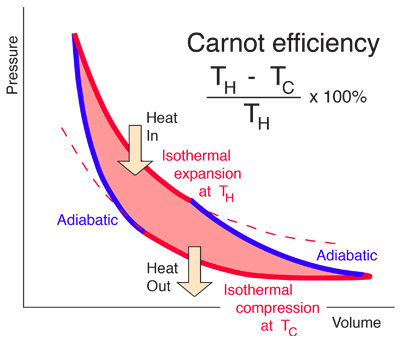
\includegraphics[scale=0.5]{carnot.png}
\subsection{Refrigerators}
Heat engine in reverse - simply reverse the arrows (put in work to suck out heat from the cold reservoir $Q_c$ and dump it into the hot reservoir $Q_h$. Coefficient of performance, COP is benefit$/$cost $=$ $Q_c/W$. By the first law, $Q_h=Q_c+W$ (we put \textit{in} work) so that the Coefficient of Performance becomes:
\begin{equation}
COP=\frac{Q_c}{Q_h-Q_c}
\end{equation}
By the second law, the inequalities are now reversed from previously (entropy flows in the opposite direction) so that:
\begin{equation}
\frac{Q_h}{T_h}\geq \frac{Q_c}{T_c}
\end{equation}
Which gives:
\begin{equation}
\mathrm{COP}\leq \frac{T_c}{T_h-T_c}
\end{equation}


\section{Free Energy and Chemical Thermodynamics}
\subsection{Free Energy as Available Work}
Helmholtz Free Energy: Total energy needed to create the system, minus the heat you can get from the environment for free at temperature $T$. For constant $T$:
\begin{equation}
F = U - TS, \qquad \Delta F = \Delta U - T\Delta S = Q + W - T\Delta S
\end{equation}
For constant $P$ and $T$, the work of a system is Gibbs Free Energy
\begin{equation}
G = H - TS = U - TS + PV, \qquad \Delta G = \Delta U - T\Delta S + P\Delta V = Q+W -T\Delta S + P\Delta V
\end{equation}
\textbf{INSERT PIC ON s151}

\subsection{Thermodynamic Identities}
\begin{equation}
dU = TdS - PdV + \mu dN
\end{equation}
\begin{equation}
dH = dU + PdV + VdP = TdS + VdP + \mu dN
\end{equation}
\begin{equation}
dF = dU - TdS - SdT = - SdT - PdV + \mu dN
\end{equation}
\begin{equation}
S = -\pd{F}{T}{V,N}, \qquad P = -\pd{F}{V}{T,N},\qquad \mu = \pd{F}{N}{T,V}
\end{equation}
\begin{equation}
dG = - SdT + VdP + \mu dN
\end{equation}
\begin{equation}
S = -\pd{G}{T}{P,N}, \qquad V = -\pd{G}{P}{T,N},\qquad \mu = \pd{G}{N}{T,P}
\end{equation}

These identities is correct if the process is reversible. Then the first law $dE = dU = Q + W$ holds.
\subsection{ Free Energy as a Force towards Equilibrium}
\begin{equation}
dS_{total} = dS + dS_R, \qquad dS = \frac{1}{T}dU  + \frac{P}{T}dV - \frac{\mu}{T}dN
\end{equation}
$dS_R = dU_T/T_R$
\begin{equation}
dS_{total} = dS + \frac{1}{T_R}dU_R
\end{equation}
$dU_R = - dU$
\begin{equation}
dS_{total} = dS - \frac{1}{T}dU = -\frac{1}{T}(dU - TdS) =-\frac{1}{T}dF
\end{equation}
This is for constant $T$, $V$ and $N$. For constant $P$
\begin{equation}
dS_{total}=-\frac{1}{T}dG
\end{equation}
\subsection{Extensive and Intensive Quantities}
Double the amount of stuff: Quantities that doubles are extrinsic; those who do not are intensive. \textbf{Extensive}: V, N, S, U, H, F, G, mass. \textbf{Intensive}: T, P, $\mu$, density. Extensive$\times$intensive = extensive. Extensive$\times$extensive = neither. Type$\times$same type = same type. Extensive $+$ intensive is not allowed.
\subsection{Gibbs Free Energy and Chemical Potential}
Given constant $T$ and $P$ we have that
\begin{equation}
\mu = \pd{G}{N}{T,P} \Rightarrow G = N\mu \text{ or } G = \sum_i N_i \mu_i
\end{equation}
\begin{equation}
\Rightarrow\frac{\partial \mu}{\partial P} = \frac{\partial}{\partial P}\frac{G}{N} = \frac{V}{N} = \frac{kT}{P}
\end{equation}
Integrating
\begin{equation}
\mu(T,P) = \mu^\circ(T,P) + kT \ln\frac{P}{P^\circ}
\end{equation}
$P^\circ$ is the atmospheric pressure, and $\mu^\circ$ is $\mu$ at this pressure and can be found in tables for for atmospheric pressures ($\mu = G/N$).  For a mixture $P$ is the partial pressure of that gas.

\subsection{Phase Transformations of Pure Substances}
\textbf{Vapor pressure}: Pressure at which a gas can coexist with its solid or liquid phase. \textbf{Triple point}: Point where all three phases can coexist. \textbf{Critical Point}: No longer a discontinuous change from liquid to gas. \textbf{Curie Temperature}: Temperature where magnetization disappears, so the phase boundary ends at a critical temperature.

\subsection{Chemical Equilibrium}
Equilibrium condition: Gibb's free energy minimized (if at room temperature and atmospheric pressure), i.e. $dG=\sum_i \mu_idN_i=0$. Generally: replace species by chemical potential, keep stochiometric ratio. Example:
\begin{equation}
N_2+3H_2 \leftrightarrow 2NH_3 \implies \mu_{N_2}+3\mu_{H_2}=2\mu_{NH_3}
\end{equation}
\subsubsection{Gaseous:}
Nitrogen fixation, $N_2+3H_2 \leftrightarrow 2NH_3$. Assume ideal gas, use $\mu_{N_2}=\mu^o_{N_2}+kT\ln\left(P_{N_2}/P_0\right)$, where $\mu_0$ is the chemical potential when its partial pressure is $P_0$. Gather all $\mu_0$ on one side, and multiply through by $N_A$ to get $\Delta G^o$. Get:
\begin{equation}
\frac{P^2_{NH_3}(P^o)^2}{P_{N_2}P^3_{NH_3}}=K=e^{-\Delta G^o/RT}
\end{equation}
Where each pressure is raised to the power of its stochiometric coefficient and there are enough powers of $P^o$ to make the expression unitless.
\subsection{Disassociation:}
$H_2O\leftrightarrow H^++OH^-$. Use $\mu^o_{H_2O}=\mu^o_{H^+}+kT\ln m_{H^+}+\mu_{OH^-}^o + kT\ln m_{OH^-}$ assuming the disassociation is small and $m$ is the molality (mole solute per kilogram solvent). Get:
\begin{equation}
m_{H^+}m_{OH^-}=e^{-\Delta G^o/RT}
\end{equation}
Where the standard states are 1 molal.
\subsection{Oxygen dissolving:}
$O_2(g)\leftrightarrow O_2(aq)$.
Use $\mu_{gas}^o+kT\ln(P/P^o)=\mu_{solute}^o+kT\ln m$ to get:
\begin{equation}
\frac{m}{P/P^o}=e^{-\Delta G_0/RT}
\end{equation}
\subsection{Ionization of hydrogen}
$H\leftrightarrow p+e$. Treat all as ideal gases, use equation \ref{eq:IdealGasMu}. Put in ionization energy $I$ explicitly, so that $\mu_H=\mu-I$ where $\mu$ is from equation \ref{eq:IdealGasMu} and $I$ is $13.6$ eV. Use ideal gas law to express with pressure, use that mass of proton and hydrogen are approximately equal, and get:
\begin{equation}
\frac{P_p}{P_H}=\frac{kT}{P_e}\left(\frac{2\pi m_e kT}{h^2}\right)^{3/2} e^{-I/kT} \quad (\mathrm{Saha\ equation})
\end{equation}
Note that $P_e/kT=N_e/V$.

\subsection{Diamonds and Graphite}
\textbf{At a given temperature and pressure, the stable phase is always the one with the lower Gibbs free energy}

To find the most stable state, use:
\begin{equation}
\pd{G}{V}{T,N} = V, \qquad \pd{G}{T}{P,N} = -S
\end{equation}
Since graphite has more volume and entropy its Gibbs free energy increases more with pressure and decreases more with temperature. Thus raising the pressure makes diamonds more stable, and with higher temperature higher pressure is needed.
\subsection{Clausius-Clapeyron Relation}
\begin{equation}
G_l = G_g
\end{equation}
at phase boundary. $dG_l = dG_g$ to remain at phase boundary. Thus
\begin{equation}
-S_ldT + V_ldP = -S_gdT + V_gdP
\end{equation}
\begin{equation}
\Rightarrow \frac{dP}{dT} = \frac{S_g - S_l}{V_g - V_l} = \frac{L}{T\Delta V}
\end{equation}
using the (total) latent heat $S_g - S_l = L/T$ and $V_g - V_l = \Delta V$. This is the Clausius-Clapeyron Relation.
\begin{equation}
\frac{dP}{dT} = \frac{\Delta S}{\Delta V} \Rightarrow \Delta V T \frac{dp}{dT} = l
\end{equation}
$l = L/N$ vapor heat per particle	

\subsection{The van der Waals Model}
\begin{equation}
\left( P + \frac{aN^2}{V^2}\right)(V-Nb) = NkT
\end{equation}
\begin{equation}
\text{total potential pressure} = -\frac{aN^2}{V} \Rightarrow P_{\text{due to p.e.}} = -\frac{d}{dV}\left(-\frac{aN^2}{V}\right) = -\frac{aN^2}{V^2}
\end{equation}
attractive force: $NkT/(V-Nb)$:
\begin{equation}
P = \frac{NkT}{V - Nb} -\frac{aN^2}{V^2}
\end{equation}
\begin{equation}
G = -NkT\ln(V-Nb) + \frac{(NkT)(Nb)}{V-Nb}- \frac{2aN^2}{V} + c(T)
\end{equation}
\begin{equation}
0 = \int_{loop} dG = \int_{loop}\pd{G}{P}{T} dP = \int_{loop} V dP 
\end{equation}
\begin{equation}
V_c = 3Nb,\qquad P_c = \frac{1}{27}\frac{a}{b^2}, \qquad kT_c = \frac{8}{27}\frac{a}{b}
\end{equation}
\subsection{Chemical Equilibrium}
\begin{equation}
0 = dG = \sum_i \mu_i dN_i
\end{equation}
\textbf{Le Chatelier's Principle}: When you disturb a system in equilibrium,it will respond in a way that partially offsets the disturbance.
\subsection{Ionization of Hydrogen}
\begin{equation}
H \leftrightarrow p + e
\end{equation}
Saha equation:
\begin{equation}
\frac{P_p}{P_H} = \frac{kT}{P_e}\left(\frac{2\pi m_e kT}{h^2}\right)^{3/2}e^{-I/kT}
\end{equation}

\section{Boltzmann Statistics}
\begin{equation}
\text{Boltzmann factor} = e^{-E(s)/kT}
\end{equation}
\begin{equation}
\mathcal{P}(s) = \frac{1}{Z}e^{-E(s)/kT},\qquad Z = \sum_s e^{-E(s)/kT}
\end{equation}
\begin{equation}
\bar{E} = \frac{1}{N}\sum_s E(s)N(s) = \sum_s E(s) \mathcal{P}(s) = \frac{1}{Z}\sum_s E(s) e^{-\beta E(s)}
\end{equation}
with $\beta = 1/kT$
\begin{equation}
\bar{E} = -\frac{1}{Z}\frac{\partial Z}{\partial \beta} = -\frac{\partial}{\partial \beta}\ln Z, \qquad U = N\bar{W}
\end{equation}
\subsection{Rotation of Diatomic Molecules}
\begin{equation}
E(j) = j(j+1)\epsilon, \qquad Z_{rot} = \sum_{j=0}^{\infty}(2j+1)e^{-E(j)/kT} = \sum_{j=0}^{\infty}(2j+1)e^{-j(j+1)\epsilon/kT}
\end{equation}
$(2j+1)$ being the degeneration.
\begin{equation}
Z_{rot} \approx \int_{0}^{\infty}(2j+1)e^{-j(j+1)\epsilon/kT} dj = \frac{kT}{\epsilon}
\end{equation}
and $kT/2\epsilon$ for identical atoms ($N_2$, $O_2$ etc).
\subsection{Equipartition Theorem}
Holds for systems where the energy is in the form of quadratic degrees of freedom $E(q) = cq^2$, where c is a constant and $q$ is some variable (coordinate, momentum, etc).
\begin{equation}
Z = \sum_q e^{-\beta E(q)} = \sum_q e^{-\beta cq^2} = \frac{1}{\Delta q}\sum_q e^{-\beta cq^2} \Delta q 
\end{equation}
\begin{equation}
\Rightarrow \frac{1}{\Delta q}\int_{-\infty}^\infty e^{-\beta cq^2} d q =\frac{1}{\Delta q}\frac{1}{\sqrt{\beta c}}\int_{-\infty}^\infty e^{-x^2} d x = C\beta ^{-1/2}
\end{equation}
\begin{equation}
\Rightarrow \bar{E} = -\frac{1}{Z}\frac{\partial Z}{\partial \beta} = \frac{1}{2}kT
\end{equation}
Lennard-Jones:
\begin{equation}
u(x) = u_0\left[\left(\frac{x_0}{x}\right)^{12} - 2\left(\frac{x_0}{x}\right)^{6}\right]
\end{equation}
\subsection{Maxwell Speed Distribution}
\begin{equation}
v_{rms} = \sqrt{\frac{2kT}{m}}
\end{equation}
\begin{equation}
\mathcal{D}(v) = \left(\frac{m}{2\pi kT}\right)^{3/2}4\pi v^2 e^{-mv^2/2kT},\qquad v_{max} = \sqrt{\frac{2kT}{m}}
\end{equation}
\begin{equation}
\bar{v} = \sum_{\text{all v}} v \mathcal{D}(v)dv = \sqrt{\frac{8kT}{\pi m}}
\end{equation}
By turning this to an integral. This is a distribution to to get probability$(v>x)$ just integrate this from $x$ to $\infty$.
\subsection{Partition Functions and Free Energy}
\begin{equation}
F = -kT\ln Z,\qquad Z = e^{-F/kT}
\end{equation}
\begin{equation}
S = -k\sum_s\mathcal{P}(s) \ln \mathcal{P}(s)
\end{equation}
\subsection{Partition Functions for Composite Systems}
For noninteracting, distinguishable particles
\begin{equation}
Z_{total} = Z_1Z_2\ldots Z_N
\end{equation}
For noninteracting, indistinguishable particles
\begin{equation}
Z_{total} =\frac{1}{N!} Z_1^N
\end{equation}
\\
Given a system with $N_A$ A-particles and $N_B$ B-particles, with $N = N_A + N_B$. The partition function becomes

\begin{equation}
Z = \binom{N}{N_A}Z_A^{N_A}Z_B^{N_B}
\end{equation}

\subsection{Ideal Gas Revisited}
\begin{equation}
Z =\frac{1}{N!} Z_1^N, \qquad Z_1 = Z_{tr}Z_{int}
\end{equation}
Where $E_{tr}$ is the transitional kinetic energy and $E_{int}$ is the internal energy (rotational, vibrational. etc). Particle in box:
\begin{equation}
\lambda_n = \frac{2L}{n}, \qquad p_n = \frac{h}{\lambda_n},\qquad E_n = \frac{p_n^2}{2m} = \frac{h^2n^2}{8mL^2}
\end{equation}
\begin{equation}
Z_{1D} = \sum_ne^{-E_n/kT} = \sum_n e^{-h^2n^2/8mL^2kT}
\end{equation}
Doing this as an integration from $0$ to $\infty$ we get
\begin{equation}
Z_{1D} = \sqrt{\frac{2\pi mk T}{h^2}}L = \frac{L}{\ell_Q} \Rightarrow \ell_Q = \frac{h}{\sqrt{\pi mkT}} 
\end{equation}
Quantum length.
\begin{equation}
Z_{tr} = \frac{L_x}{\ell_Q}\frac{L_y}{\ell_Q}\frac{L_z}{\ell_Q} = \frac{V}{v_Q}
\end{equation}
\begin{equation}
\Rightarrow Z_1 = \frac{V}{v_Q}Z_{int}\Rightarrow Z = \frac{1}{N!}\left(\frac{VZ_{int}}{v_Q}\right)^N,\qquad \ln Z = N( \ln V + \ln Z_{int} - \ln N - \ln v_Q + 1)
\end{equation}
\begin{equation}
U = \frac{\partial}{\partial \beta} Z =  U_{int} + \frac{3}{2}NkT 
\end{equation}
\begin{equation}
C_V = \frac{\partial U}{\partial T} = \frac{\partial U_{int}}{\partial T} + \frac{3}{2}Nk
\end{equation}
\begin{equation}
F = -kT\ln Z = -NkT(\ln V - \ln N - \ln v_Q + 1) + F_{int}
\end{equation}
\begin{equation}
S = Nk\left[\ln \left(\frac{V}{Nv_Q}\right) + \frac{5}{2}\right] - \frac{\partial F_{int}}{\partial T}, \qquad P = \frac{NkT}{V},\qquad \mu = -kT\ln \frac{V Z_{int}}{Nv_Q}
\end{equation}
\section{Quantum Statistics}
\subsection{Gibbs Factor}
For a system i thermal and diffusive contact with a much larger reservoir, whose temperature and chemical potential are effectively constant.
\begin{equation}
\text{Gibbs Factor} = e^{-(E(s) - \mu N(s))/kT}
\end{equation}
\begin{equation}
\mathcal{P}(s) = \frac{1}{\mathcal{Z}}e^{-(E(s) - \mu N(s))/kT}, \qquad \mathcal{Z} = \sum_s e^{-(E(s) - \mu N(s))/kT}
\end{equation}
$\mathcal{Z}$ is the grand partition function.
\subsection{Bosons and Fermions}
\subsubsection{Fermions:  Fermi-Dirac distribution}
On states allowed are $0$ and $1$
\begin{equation}
\mathcal{Z} = 1 + e^{-(\epsilon - \mu)/kT} \Rightarrow \bar{n} = \sum_n n \mathcal{P}(n) = 0\cdot\mathcal{P}(0) + 1\cdot\mathcal{P}(1) = \frac{1}{1 + e^{(\epsilon - \mu)/kT}}
\end{equation}
\subsubsection{Bosons: Einstein-Bose distribution}
All states allowed
\begin{equation}
\mathcal{Z} = 1 + e^{-(\epsilon - \mu)/kT} + e^{-2(\epsilon - \mu)/kT}\ldots = 1 + e^{-(\epsilon - \mu)/kT} + \left( e^{-(\epsilon - \mu)/kT}\right)^2\ldots =\frac{1}{1 - e^{-(\epsilon - \mu)/kT}}
\end{equation}

\begin{equation}
\bar{n} = \sum_n n \mathcal{P}(n) = -\frac{1}{\mathcal{Z}}\frac{\partial \mathcal{Z}}{\partial x} = \frac{1}{1-e^{(\epsilon - \mu)/kT}}
\end{equation}
Where $x = (\epsilon - \mu)/kT$. For reference: for the Boltzmann distribution
\begin{equation}
\bar{n}_{boltzmann} = N\mathcal{P}(s) = \frac{N}{Z_1}e^{-\epsilon/kT} = e^{-(\epsilon-\mu)/kT}
\end{equation}
Using $\mu = -kT\ln (Z_1/N)$
\subsection{Degenerated Gas}
For Boltzmann statistics to apply $V/N>> v_Q$. Classical limit $(\epsilon - \mu=/kT >> 1$. Then we can ignore the $1$ in the FD distribution.	
\subsubsection{Zero Temperature}
\begin{equation}
\epsilon_F = \mu(T = 0)
\end{equation}
Particle in box:
\begin{equation}
\epsilon = \frac{|\vec{p}|^2}{2m} = \frac{h^2}{8mL^2}(n^2_x + n^2_y + n^2_z)
\end{equation}
\begin{equation}
\epsilon_F = \frac{h^2n_{max}^2}{8mL^2}
\end{equation}
\begin{equation}
N = 2\times \text{(volume of eighth-sphere)} = 2\frac{1}{8}\cdot\frac{4}{3}\pi n_{max}^3 = \frac{\pi n_{max}^3}{3}
\end{equation}
With $V=L^3$
\begin{equation}
\epsilon_F = \frac{h^2}{8m}\left(\frac{3N}{\pi V}\right)^{2/3}
\end{equation}
\begin{equation}
U = 2\int \int \int \epsilon(\vec{n})dn_x dn_y dn_z = 2\int_0^{n_{max}}dn\int_0^{\pi/2}d\theta\int_0^{\pi/2}d\phi n^2\sin\theta \epsilon(n) = \frac{3}{5}N\epsilon_F
\end{equation}
\begin{equation}
T_F = \frac{\epsilon_F}{k}, \qquad P = \frac{2N\epsilon_F}{5V} = \frac{2U}{3V}
\end{equation}
Degeneracy pressure. Bulk modulus
\begin{equation}
B = -V\pd{P}{V}{T} = \frac{10U}{9V}
\end{equation}
\subsubsection{Low Temperature}
\begin{equation}
U = \frac{3}{5}N\epsilon_F + \frac{\pi^2}{4}N\frac{(kT)^2}{\epsilon_F}, \qquad C_V = \frac{\pi^2 Nk^2T}{2\epsilon_F}
\end{equation}
\subsubsection{Density of States}
\begin{equation}
\epsilon = \frac{h^2}{8mL^2}n^2 \Rightarrow n = \sqrt{\frac{8mL^2}{h^2}}\sqrt{\epsilon} \Rightarrow dn = \sqrt{\frac{8mL^2}{h^2}} \frac{1}{2\sqrt{\epsilon}}d\epsilon
\end{equation}
From
\begin{equation}
U = \pi \int_0^{n_{max}}\epsilon(n) n^2 dn
\end{equation}
We get
\begin{equation}
U = \int_0^{\epsilon_F}\epsilon\left[\frac{\pi}{2}\left(\frac{8mL^2}{h^2}\right)^{3/2}\sqrt{\epsilon}\right] d\epsilon
\end{equation}
at $T=0$
\begin{equation}
g(\epsilon) = \frac{\pi}{2}\frac{(8m)^{3/2}}{h^3}V\sqrt{\epsilon} = \frac{3N}{2\epsilon_F^{3/2}}\sqrt{\epsilon}
\end{equation}
For $T=0$ we then get
\begin{equation}
N = \int_0^{\epsilon_F}g(\epsilon) d\epsilon
\end{equation}
and for any $T$ we get
\begin{equation}
N = \int_0^{\epsilon_F}g(\epsilon) \bar{n}_{FD}(\epsilon) d\epsilon \int_0^{\epsilon_F}g(\epsilon)\frac{1}{1 + e^{(\epsilon - \mu)/kT}} d\epsilon
\end{equation}
\begin{equation}
U = \int_0^{\epsilon_F}\epsilon g(\epsilon) \bar{n}_{FD}(\epsilon) d\epsilon \int_0^{\epsilon_F}\epsilon g(\epsilon)\frac{1}{1 + e^{(\epsilon - \mu)/kT}} d\epsilon
\end{equation}
and for $T\neq 0 \Rightarrow \mu(T) \neq \epsilon_F$
\subsubsection{Sommerfeld Expansion}
\begin{equation}
\frac{\mu }{\epsilon_F} = 1 - \frac{\pi^2}{12}\left(\frac{kT}{\epsilon_F}\right)^2 + \ldots
\end{equation}
\begin{equation}
U = \frac{3}{5}N\epsilon_F + \frac{\pi^2}{4}N\frac{(kT)^2}{\epsilon_F} + \ldots
\end{equation}
\subsection{Blackbody radiation}
Ultraviolet catastrophe: theoretically one expected infinite wavelengths with $E = 2\cdot 1/2 kT$, but this was not the case experimentally.

\subsubsection{Planck Distribution}
\begin{equation}
E_n = 0,hf,2hf,\ldots \Rightarrow Z = 1 + e^{-\beta ht} + e^{-2\beta hf}+ \ldots = \frac{1}{1-e^{-\beta hf}}
\end{equation}
\begin{equation}
\bar{E} = - \frac{1}{Z}\frac{\partial Z}{\partial \beta} = \frac{hf}{e^{hf/kT} - 1}, \qquad \bar{n}_{Pl} = \frac{1}{e^{hf/kT} - 1}
\end{equation}
\subsubsection{Photons}
Use the Einstein-Bose distribution. And:
\begin{equation}
\mu = 0
\end{equation}
since
\begin{equation}
\pd{F}{N}{T,V} = 0
\end{equation}
at equilibrium. This i s because the number of photons $N$ is not constrained but takes what ever value minimizes $F$. So a small $dN$ should leave $F$ untouched.
\subsubsection{Summing over Modes}
\begin{equation}
\lambda = \frac{2L}{n}, \qquad p = \frac{hn}{2L},\Rightarrow e\epsilon = pc = \frac{hcn}{2L}
\end{equation}
\begin{equation}
U = 2\int_0^{\infty}dn\int_0^{\pi/2}d\theta\int_0^{\pi/2}d\phi n^2\sin\theta \frac{hcn}{2L}\frac{1}{e^{hcn/2LkT}-1}
\end{equation}
\subsubsection{Planck Spectrum}
changing variables to $\epsilon = hcn/2L$
\begin{equation}
\frac{U}{V} = \int_0^\infty \frac{8\pi\epsilon^3/(hc)^3}{e^{\epsilon/kT}-1} d\epsilon
\end{equation}
The energy density per unit photon energy or the spectrum is
\begin{equation}
u(\epsilon) = \frac{8\pi}{(hc)^3}\frac{\epsilon^3}{e^{\epsilon/kT}-1}
\end{equation}
with $x = \epsilon/kT$
\begin{equation}
\frac{U}{V} = \frac{8\pi(kT)^4}{(hc)^3}\int_0^\infty\frac{x^3}{e^x - 1} dx
\end{equation}
\subsubsection{Total Energy}
\begin{equation}
\frac{U}{V} = \frac{8\pi^5(kT)^4}{15(hc)^3}
\end{equation}
\subsubsection{Entropy of Photon Gas}
\begin{equation}
C_V = \pd{U}{T}{V} = 4aT^3
\end{equation}
$a = 8\pi^5k^4V/15(hc)^3$
\begin{equation}
S(T) = \int_0^T\frac{C_V(T)}{T}dT = \frac{4}{3}aT^3
\end{equation}
\subsubsection{Photons Escaping Though a Hole}
Stefan-Boltzmann constant $\sigma$. Stefan's Law:
\begin{equation}
\text{power per unit area} = \frac{2\pi^5}{15}\frac{(kT)^4}{h^3c^2} = \sigma T^4
\end{equation}
\subsection{Blackbody Radiation}
Ultraviolet catastrophe: Each mode in the field has energy $kT$, infinite number of modes, infinite energy. Solution: $E_n=nhf$, $n\in \mathbb{N}^+$. For a single oscillator then:
\begin{equation}
Z=1+e^{-\beta hf}+e^{-2\beta hf}+...=\frac{1}{1-e^{-\beta hf}}\quad \overline{E}=\frac{hf}{e^{hf/kT}-1}
\end{equation}
Average number of "units of energy" (photons) in a single oscillator is $\overline{n}=1/(\exp(hf/kT)-1)$ (Planck Distribution). But photons are bosons, must follow Bose-Einstein $\rightarrow$ $\mu=0$ for photons (follows also because $N$ arbitrary for photons so $(\partial F/\partial N)_{T,V}=0=\mu$ or from $e\leftrightarrow e+\gamma \implies \mu_e=\mu_e+\mu_{\gamma}$). Energy for photons is $\epsilon=pc=hcn/2L$. Each wave shape can hold two photons. Gives the total energy per unit volume as:
\begin{equation}
\frac{U}{V}=\int_0^{\infty} \underbrace{\frac{8\pi \epsilon^3/(hc)^3}{\exp(\epsilon/kT)-1}}_{\mathrm{Spectrum\ of\ photon}} d\epsilon = \frac{8\pi^5(kT)^4}{15 (hc)^3}
\end{equation}
Spectrum peaks at $\epsilon=2.82 kT$ (Wien's law). Heat capacity/entropy:
\begin{equation}
C_V=4aT^3 \quad S(T)=\int_0^T \frac{C_V(T')}{T'}dT'=4aT^3 \quad N=8\pi V\left(\frac{kT}{hc}\right)^3 \int_0^{\infty} \frac{x^2}{e^x-1}dx
\end{equation}
Where $a=8\pi^5k^4V/15(hc)^3$.
\subsection{Photons Escaping through a Hole}
Spectrum outside of box with hole is same as inside, as all photons travel at the same speed. Energy comes from spherical shell, distance $R$ from hole, with angle $\theta$ to the normal of the hole. Look at chunk of spherical shell: volume $R^2 \sin \theta c\ dt d\theta d\phi$. Energy is this times $U/V$.Probability of escape is $A\cos \theta/4\pi R^2$ with $A$ aperture size. Total energy escaping:
\begin{equation}
\int_0^{2\pi}d\phi \int_0^{\pi/2} d\theta \frac{A\cos \theta}{4\pi}\frac{U}{V}cdt\sin \theta = \frac{A}{4}\frac{U}{V}cdt
\end{equation}
Which gives power per unit area as:
\begin{equation}
P=\frac{2\pi^5}{15}\frac{\left(kT\right)^4}{h^3c^2}=\sigma T^4 \ \mathrm{(Stefan-Boltzmann\ law)}
\end{equation}
If reflecting: remember to include emissitivity, $e$.
\subsection{The Sun and the Earth}
Absorbed power: solar constant$\times \pi R^2= 4\pi R^2\sigma T^4$ : emitted power.
\subsubsection{Radiation from Other Object}
\textbf{Emissivity} $e$:
\begin{equation}
\text{power} = \sigma e A T^4
\end{equation}
\subsubsection{Sun and Earth}
Luminosity: Sun $3.9\cdot 10^{6}$ watts.
\begin{equation}
T = \left(\frac{\text{luminosity}}{\sigma A}\right)^{1/4} = 5800 K \Rightarrow\epsilon = 2.82kT = 1.41 eV
\end{equation}
\begin{equation}
\epsilon = 2.82kT
\end{equation}
\begin{equation}
(\text{solar constant}) \cdot \pi R^4 = 4\pi R^2 \sigma T^4 \Rightarrow T_{earth} = 279 K
\end{equation}
Real: $288$ K

\section{Div:}
\subsection{Div:}
tilstandsliking = pressure
\begin{equation}
n = \frac{N}{V} = \frac{P}{kT},\qquad (\text{From }PV = NkT)
\end{equation}
\subsection{Maxwell's relations}
\begin{equation}
\pd{T}{V}{S} = -\pd{P}{S}{V}, \qquad \pd{T}{P}{S} = \pd{V}{S}{P}
\end{equation}
\begin{equation}
\pd{S}{V}{T} = \pd{P}{T}{V}, \qquad -\pd{S}{P}{T} = \pd{V}{T}{P}
\end{equation}
These comes from the fact that 
\begin{equation}
\pd{^2F}{x\partial y}{} = \pd{^2F}{y\partial x}{}
\end{equation}
\subsection{Ensembles}
\subsubsection{Micro canonical}
(NVU) isolated. Multiplicity $\Omega$ and entropy $S = k\ln\Omega$
\subsubsection{Canonical}
(NVT). $N$ and $V$ constant, $U$ varies.
\begin{itemize}
\item State: $Z = \sum_i e^{-\beta E(i)}$
\item $T$ in equilibrium
\item Probability $P(i) = \frac{1}{Z}e^{-\beta E_i}$
\item $\bar{E} = \frac{1}{Z}\frac{\partial Z}{\partial \beta}$
\item Helmholtz $F$
\end{itemize}
\subsubsection{Grand Canonical}
($\mu$VT)
\begin{itemize}
\item $V$ constant
\item $T$ and $\mu$ in equilibrium
\item Gibbs factor
\item $\bar{n} = \frac{kT}{\mathcal{Z}}\frac{\partial \mathcal{Z}}{\partial \beta}$
\item Grand Potential $\Phi = U - TS - \mu N = -kT\ln \mathcal{Z}$
\end{itemize}
\subsection{Div Functions}
\begin{equation}
e^x + e^{-x} = 2\cosh x
\end{equation}
\begin{equation}
P(\text{noyaktig saa mange riktige paa saa mange forsoek}) = \binom{N}{n}p^n(1-p)^{N-n}
\end{equation}

\end{document}

